\documentclass{standalone}
\usepackage{tikz}
\usepackage{verbatim}
\begin{document}
\pagestyle{empty}
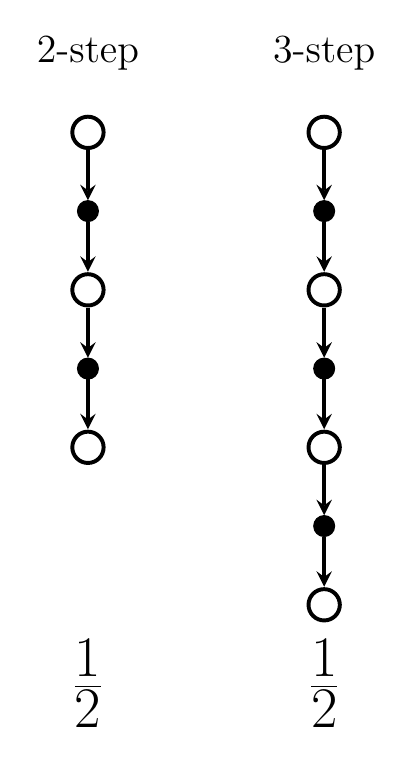
\begin{tikzpicture}

  % TD 2 step
  \node at (3, 1) {\Large 2-step};
  \node[draw,circle,scale=1.2, fill=white, line width=0.5mm] (s_3) at (3,0) {};
  \foreach \xa in {-1,-3} {
      \node[draw,circle,fill,scale=0.8] (b3\xa) at (3, \xa) {};
      \node[draw,circle,scale=1.2, fill=white,line width=0.5mm] (s3\xa) at (3,\xa-1) {};
      \draw[-stealth, line width=0.5mm] (b3\xa) -- (s3\xa);
  }
  \draw[-stealth, line width=0.5mm] (s_3) -- (b3-1);
  \draw[-stealth, line width=0.5mm] (s3-1) -- (b3-3);
  
    % TD 3 step
  \node at (6, 1) {\Large 3-step};
  \node[draw,circle,scale=1.2, fill=white, line width=0.5mm] (s_6) at (6,0) {};
  \foreach \xa in {-1,-3,-5} {
      \node[draw,circle,fill,scale=0.8] (b6\xa) at (6, \xa) {};
      \node[draw,circle,scale=1.2, fill=white,line width=0.5mm] (s6\xa) at (6,\xa-1) {};
      \draw[-stealth, line width=0.5mm] (b6\xa) -- (s6\xa);
  }
  \draw[-stealth, line width=0.5mm] (s_6) -- (b6-1);
  \draw[-stealth, line width=0.5mm] (s6-1) -- (b6-3);
  \draw[-stealth, line width=0.5mm] (s6-3) -- (b6-5);
  \node at (6, -7) {\Huge $\frac{1}{2}$};
  \node at (3, -7) {\Huge $\frac{1}{2}$};
 \end{tikzpicture}
\end{document}